\chapter{聲音、量子振子與第二定律}

\lectureoverview{第二定律是我們最終要探討的主題，但有兩個具體計算會先為此鋪路。聲速說明熱力學導數如何轉化為可觀測的運動。接著，諧振子揭示經典能量均分定理在剛性自由度上的失效，並展示量子力學如何逐一啟動各個模式。最後，我們會回到可逆的微觀動力學與熵增加之間看似矛盾之處，運用相空間流、粗粒化、混沌與迴歸，將第二定律表述為一條幾乎必然成立的定律，而非毫無例外的力學禁令。}

\section{對第二定律的承諾}

核心問題容易陳述，卻難以解釋。牛頓方程具有可逆性：若某段微觀歷程是允許的，那麼將時間反演後的歷程也同樣允許。然而，第二定律指出宏觀過程有其優先方向，通常表現為熵增加。我們會探討這個張力，但不會立刻著手。最好先看看統計力學如何得出具體結果，再透過一個初等計算，認識那個迫使經典物理讓位給量子物理的歷史謎題。

第一個例子是數值估算，而且刻意採用粗略方法：估計稀薄氣體中的聲速。第二個例子則在其假設下是精確的：計算熱浴中諧振子的平均能量。諧振子將帶我們從能量均分走向量子化能階，從單一模式走向無窮多個模式，最後再回到一個問題：多粒子系統忘卻初始狀態究竟是什麼意思？

\section{聲速的分子尺度}

想像稀薄氣體中有一小塊密度較高的區域。分子離開擁擠處，使這個區域逐漸擴散，因此其傳播速度應與分子速度相近。能量均分定理給出單一分子的動能：
\begin{equation}
 \frac{3}{2}k_B T
 =\frac{1}{2}m\expect{v^2},
 \qquad
 \expect{v^2}=\frac{3k_B T}{m}.
 \label{eq:sm7-molecular-speed}
\end{equation}
此處的溫度以絕對零度為基準；由於我們要使用實驗室單位制，因此恢復了 \(k_B\)。這個論證只能估算尺度：分子的均方根速率本身並不等於集體聲波的傳播速度。

更系統的推導會考慮一小塊氣體。相對兩面上的壓力不等，會產生淨力；氣體的加速度則與質量密度成反比。結果可寫成
\begin{equation}
 c_s^2=
 \left(\frac{\partial P}{\partial \rho_m}\right)_{\cal C},
 \qquad
 \rho_m=m\rho,
 \label{eq:sm7-sound-general}
\end{equation}
其中 \(\rho\) 是數密度，下標 \({\cal C}\) 表示擾動所遵循的熱力學條件。板書中的計算採用
\begin{equation}
 P=\rho k_B T
 \quad\Longrightarrow\quad
 \frac{1}{m}
 \left(\frac{\partial P}{\partial\rho}\right)_T
 =\frac{k_B T}{m}.
 \label{eq:sm7-sound-isothermal}
\end{equation}
這是等溫聲速的估算。其平方與 \eqref{eq:sm7-molecular-speed} 相差因子 \(3\)，也就是速度相差因子 \(\sqrt{3}\)。

\begin{figure}[t]
\centering
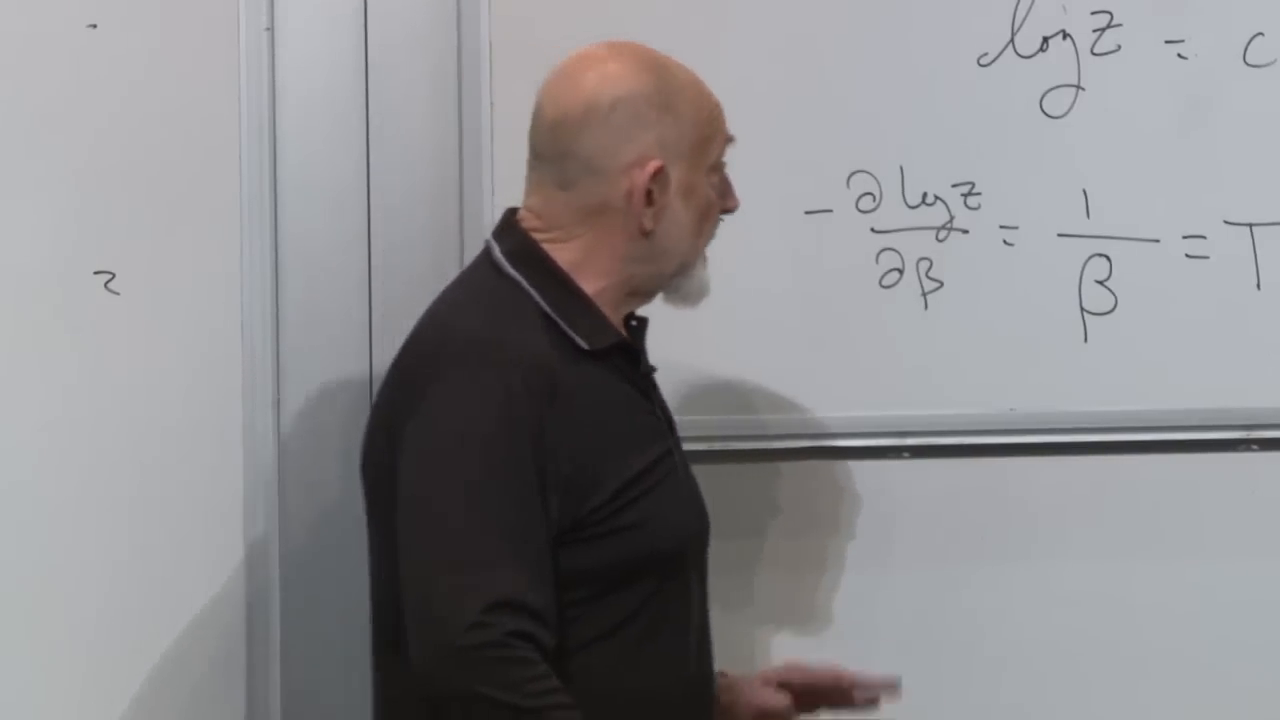
\includegraphics[width=0.90\textwidth]{lecture_07_figure_02.png}
\caption{合併展示分子速度的估算、壓力導數及理想氣體代入結果。}
\lectureframe{00:08:55}
\end{figure}

這裡還需要一項重要修正。小振幅聲波造成氣體壓縮與膨脹的速度，通常快於熱量在相鄰氣體微元之間傳遞的速度。因此，局部運動近似為絕熱，而非等溫：
\begin{equation}
 c_s^2=
 \left(\frac{\partial P}{\partial\rho_m}\right)_S.
 \label{eq:sm7-sound-adiabatic}
\end{equation}
對於絕熱指數為 \(\gamma\) 的理想氣體，
\begin{equation}
 P\rho_m^{-\gamma}=\text{constant},
 \qquad
 c_s^2=\gamma\frac{P}{\rho_m}
       =\gamma\frac{k_B T}{m}.
 \label{eq:sm7-sound-ideal-adiabatic}
\end{equation}
室溫下的雙原子空氣，其 \(\gamma\simeq 7/5\)。因此，定溫計算可作為有用的初步估算，而絕熱導數則給出物理上適用的修正。

採用以下粗略數值：
\begin{equation}
\begin{aligned}
 k_B&\simeq1.3\times10^{-23}\ {\rm J\,K^{-1}},
 &T&\simeq300\ {\rm K},\\
 m_{\rm air}&\simeq4\times10^{-26}\ {\rm kg}.&&
\end{aligned}
 \label{eq:sm7-air-data}
\end{equation}
分子速度估算值約為 \(500\ {\rm m\,s^{-1}}\)。此處的溫度必須是以開爾文表示的絕對溫度，不能使用華氏這類以偏移量為基準的溫標。熟知的聲速約為 \(300\ {\rm m\,s^{-1}}\)；絕熱理想氣體公式則在室溫下給出約 \(340\ {\rm m\,s^{-1}}\)。因此，這項粗略計算得到了正確的物理尺度。

\begin{figure}[t]
\centering
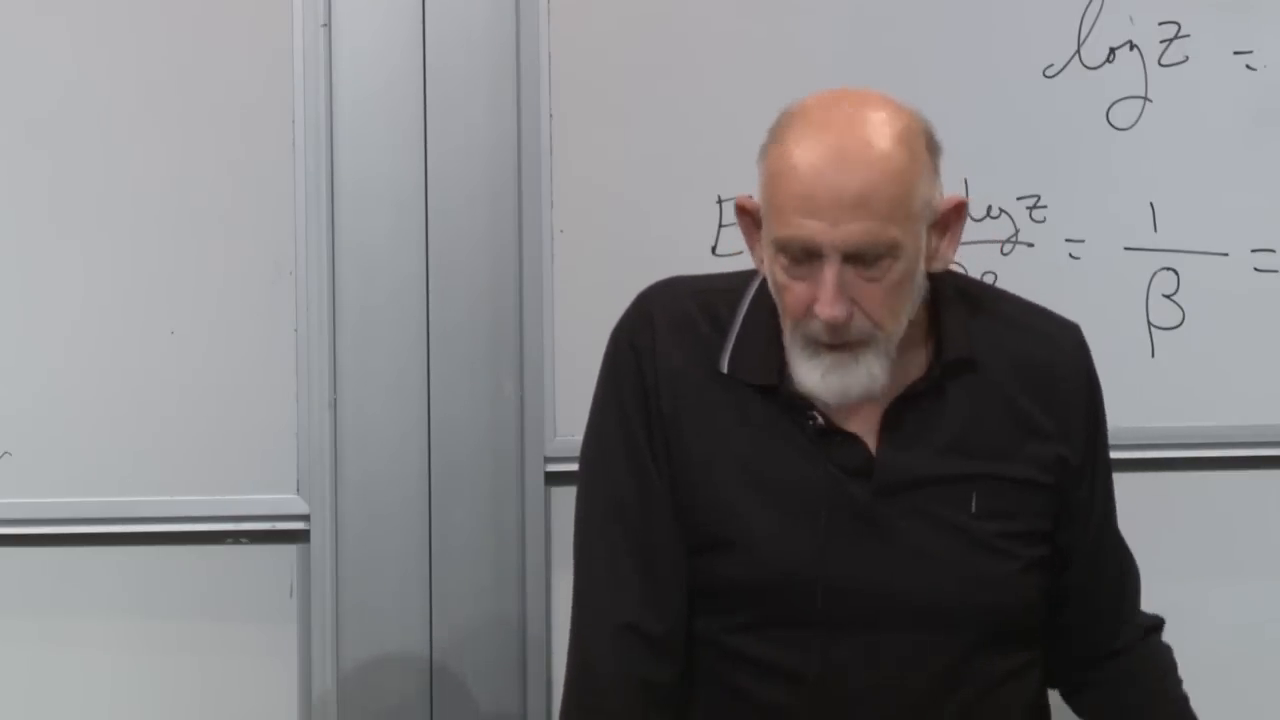
\includegraphics[width=0.90\textwidth]{lecture_07_figure_03.png}
\caption{以玻爾茲曼常數、約為 \(30\) 個質子質量的有效分子質量，以及 \(T\simeq300\ {\rm K}\)，估算室溫空氣中的聲速。}
\lectureframe{00:10:55}
\end{figure}

早在微觀理論尚未出現之前，人們就能藉由測量壓力隨密度的變化來求得聲速。統計力學的論證進一步提供了一個引人注目的解釋：所得的宏觀速度由單一分子的熱運動速度決定。

\begin{classroomqa}
\audiencequestion{分子質量是否應計入中子？氮的數值 \(14\) 是否只計算質子？}
\lecturerresponse{引用的原子量已將質子和中子都計入。氮分子含有兩個原子，每個原子的原子量約為 \(14\)，因此分子質量約為 \(28\) 個質子質量。就這項估算而言，將 \(28\) 約取為 \(30\) 已足夠。
\lecturetimestamp{00:10:58--00:11:16}}
\end{classroomqa}

\begin{classroomqa}
\audiencequestion{因子 \(3\) 來自三個平移方向，但聲波只沿一個方向傳播。這是否表示應該去掉因子 \(3\)？}
\lecturerresponse{這個問題提醒我們，不應把三維的分子均方根速率等同於一維的傳播速率。前面的論證只是數量級估算。要得到受控的結果，應使用壓力導數，並採用適用於該波的熱力學條件。
\lecturetimestamp{00:11:12--00:12:00}}
\end{classroomqa}

\begin{classroomqa}
\audiencequestion{這個導數是否假設波傳播時溫度保持不變？}
\lecturerresponse{是的，展示的理想氣體代入式採用了這項假設。對極小的擾動而言，定溫是合理的初步估算；標準修正則是將一般聲波視為近似絕熱，並以 \(\left(\partial P/\partial\rho_m\right)_S\) 取代等溫導數。
\lecturetimestamp{00:12:59--00:14:01}}
\end{classroomqa}

\begin{classroomqa}
\audiencequestion{如果壓力和密度的變化都很小，它們的導數是否也會很小？}
\lecturerresponse{不會。導數是在無窮小極限下兩個小變化量的比值。\(\delta P\) 和 \(\delta\rho\) 都可能很小，但 \(\delta P/\delta\rho\) 仍可維持有限，並決定波速。
\lecturetimestamp{00:14:03--00:14:23}}
\end{classroomqa}

\begin{classroomqa}
\audiencequestion{氣體受到壓縮時，聲速是否應該提高，就像物質從氣體轉變為液體或固體時那樣？}
\lecturerresponse{是。導數是在所考慮的狀態下計算的，而 \(P(\rho,T)\) 不一定是線性函數。分子被擠得彼此靠近時，狀態方程會偏離理想氣體形式，\(\partial P/\partial\rho\) 也可能大幅增加。
\lecturetimestamp{00:14:25--00:15:13}}
\end{classroomqa}

\begin{classroomqa}
\audiencequestion{數值 \(500\ {\rm m\,s^{-1}}\) 能否用於任意壓力？}
\lecturerresponse{不能。這個數值適用於低密度範圍，因為在此範圍內理想氣體方程是有用的近似。一旦 \(P(\rho,T)\) 中出現密度的高次項，導數因而聲速，就會隨壓力和密度而變化。
\lecturetimestamp{00:15:14--00:16:29}}
\end{classroomqa}

\begin{classroomqa}
\audiencequestion{密度增加時，聲波以約略等於分子速度的速度傳播這個原先的圖像，是否也會失效？}
\lecturerresponse{很可能會。這個圖像是針對稀薄氣體提出的。密度高時，集體交互作用會變得愈來愈重要；這正是狀態方程的導數能提供更一般描述的原因。
\lecturetimestamp{00:16:32--00:16:53}}
\end{classroomqa}

\begin{classroomqa}
\audiencequestion{為什麼氮分子的質量寫成約 \(30\) 個質子質量，而不是 \(28\)？}
\lecturerresponse{這項估算只需要相稱的數值精度，因此將 \(28\) 約取為 \(30\)。原先的 \(500\ {\rm m\,s^{-1}}\) 估算值除以 \(\sqrt{3}\simeq1.7\) 後也接近 \(300\ {\rm m\,s^{-1}}\)，不過要計算修正量，仍應採用絕熱導數這種受控的方法。
\lecturetimestamp{00:16:54--00:17:27}}
\end{classroomqa}

\section{熱浴中的單一經典振子}

現在，我們以單一諧振子取代自由平移的分子，並把其他一切視為熱浴。彈簧上掛著質量塊，是最直接的例子，但這個模型的適用範圍更廣。電磁腔中的模式會振盪；晶體中的原子會振盪；幾乎任何穩定系統只要稍微偏離平衡，在最低階近似下都會作簡諧運動。

令 \(x\) 表示相對於平衡位置的位移，動量為 \(p\)、質量為 \(m\)，彈簧常數為 \(\kappa\)，則哈密頓量為
\begin{equation}
 H(x,p)=\frac{p^2}{2m}+\frac{\kappa x^2}{2},
 \qquad
 \omega=\sqrt{\frac{\kappa}{m}}.
 \label{eq:sm7-classical-hamiltonian}
\end{equation}
熱浴決定 \(T\)；從此處起，我們再次採用 \(k_B=1\)，因此 \(\beta=1/T\)。與室溫環境達到平衡的振子，其溫度約為 \(300\ {\rm K}\)；浸在液態氦中的振子，溫度則只有幾開爾文。假想的彈簧若置於太陽中心，便無法維持彈簧的狀態，但這個例子清楚說明了環境的作用。玻爾茲曼權重可分解為
\begin{equation}
 e^{-\beta H}
 =e^{-\beta p^2/(2m)}
  e^{-\beta\kappa x^2/2}.
 \label{eq:sm7-factorized-weight}
\end{equation}

\begin{figure}[t]
\centering
\includegraphics[width=0.90\textwidth]{lecture_07_figure_04.png}
\caption{彈簧質量振子，以及由動能和位能組成的哈密頓量。}
\lectureframe{00:20:55}
\end{figure}

與自由氣體不同，位置積分不只是給出容器體積。回復力位能會對每個位移加權：
\begin{equation}
 Z_{\rm cl}
 =\frac{1}{h}\int_{-\infty}^{\infty}dp
             \int_{-\infty}^{\infty}dx\,
 e^{-\beta p^2/(2m)}
 e^{-\beta\kappa x^2/2}.
 \label{eq:sm7-classical-z}
\end{equation}
因子 \(1/h\) 使一維經典配分函數成為無因次量。板書計算中省略了這個因子，因為它與 \(\beta\) 無關，也不會影響平均能量。

\begin{figure}[t]
\centering
\includegraphics[width=0.90\textwidth]{lecture_07_figure_05.png}
\caption{經典振子的配分函數分解為動量與位移兩個高斯積分。}
\lectureframe{00:22:55}
\end{figure}

對動量積分，令
\begin{equation}
 q=\sqrt{\frac{\beta}{2m}}\,p,
 \qquad
 dp=\sqrt{\frac{2m}{\beta}}\,dq.
 \label{eq:sm7-p-gaussian-substitution}
\end{equation}
對位置積分，令
\begin{equation}
 y=\sqrt{\frac{\beta\kappa}{2}}\,x,
 \qquad
 dx=\sqrt{\frac{2}{\beta\kappa}}\,dy.
 \label{eq:sm7-x-gaussian-substitution}
\end{equation}
由於 \(\int_{-\infty}^{\infty}e^{-u^2}\,du=\sqrt{\pi}\)，板書中使用的未歸一化相空間積分為
\begin{equation}
 \int dp\,dx\,e^{-\beta H}
 =\frac{2\pi}{\beta}\sqrt{\frac{m}{\kappa}}
 =\frac{2\pi}{\beta\omega}.
 \label{eq:sm7-classical-z-unnormalized}
\end{equation}
恢復相空間胞元後，得到
\begin{equation}
 Z_{\rm cl}=\frac{2\pi}{h\beta\omega}
           =\frac{1}{\beta\hbar\omega}.
 \label{eq:sm7-classical-z-normalized}
\end{equation}

只有對能量有影響的 \(\beta\) 依賴部分：
\begin{equation}
 \begin{aligned}
 \log Z_{\rm cl}&=\text{constant}-\log\beta,\\
 \expect{H}
 &=-\frac{\partial\log Z_{\rm cl}}{\partial\beta}\\
 &=\frac{1}{\beta}=T.
 \end{aligned}
 \label{eq:sm7-classical-energy}
\end{equation}

\begin{figure}[t]
\centering
\includegraphics[width=0.90\textwidth]{lecture_07_figure_06.png}
\caption{右側黑板上的完整經典推導：高斯積分的因式分解、\(Z\propto(\beta\omega)^{-1}\)，以及 \(\expect{H}=1/\beta=T\)。}
\lectureframe{00:30:15}
\end{figure}

這裡沒有因子 \(3\)，因為只有一個空間維度的振子。也沒有剩下因子 \(1/2\)，因為哈密頓量包含兩個獨立的二次項。每個高斯積分都貢獻 \(T/2\)：
\begin{equation}
 \expect{K}=\frac{T}{2},
 \qquad
 \expect{U}=\frac{T}{2},
 \qquad
 \expect{H}=T.
 \label{eq:sm7-equipartition-oscillator}
\end{equation}
這是最實用的能量均分形式：經典哈密頓量中的每個獨立二次項都貢獻 \(T/2\)。

答案與 \(m\) 和 \(\kappa\) 都無關，但運動本身確實取決於這兩個參數：
\begin{equation}
 \expect{p^2}=mT,
 \qquad
 \expect{x^2}=\frac{T}{\kappa},
 \qquad
 \expect{\dot{x}^2}=\frac{T}{m}.
 \label{eq:sm7-classical-fluctuations}
\end{equation}
因此，質量較大的物體運動較慢，彈簧較硬時振幅較小，但平均能量仍為 \(T\)。當 \(\kappa\) 大得驚人時，這個結果便令人不安。硬到幾乎無法運動的彈簧，理應如同凍結的約束；然而經典能量均分定理仍賦予它 \(T\) 的能量。

\begin{classroomqa}
\audiencequestion{當 \(\kappa\to\infty\) 時，配分函數趨近於零。為什麼仍然可以使用它的對數？}
\lecturerresponse{讓 \(\kappa\) 保持有限，但可以任意大。它對 \(\log Z\) 的貢獻是加法項，且與 \(\beta\) 無關，因此對 \(\beta\) 微分仍會得到 \(T\)。這種極限情況帶來的不安確實存在：經典計算本身邏輯一致，但它漏掉了自然界中一項對極硬振子不可或缺的特性。
\lecturetimestamp{00:34:01--00:34:54}}
\end{classroomqa}

\begin{classroomqa}
\audiencequestion{理想氣體的配分函數需要一個 \(N!\)。這裡是否也應該有類似的階乘？}
\lecturerresponse{不需要。我們研究的是一個指定的振子，而不是排列 \(N\) 個全同粒子。若有許多彼此獨立且各自可辨識的模式，配分函數就彼此相乘。不可區分性因子適用於另一種計數問題。
\lecturetimestamp{00:35:03--00:35:40}}
\end{classroomqa}

\section{經典能量均分為何成了一場危機}

真實分子並非沒有結構的點粒子。雙原子分子包含可振動的化學鍵，因此具有內部振子。若按經典理論直接計數，即使在一般溫度下，也會把額外的熱能分配給這個模式。以刻意簡化的示意性計算來說，啟動一個振動模式，會使能量從 \(3T/2\) 提高到接近 \(5T/2\)。若要精確計算熱容量，還必須納入轉動自由度，並區分能量與能量對溫度的導數。更直接的關鍵實驗事實是：低溫下，剛性的內部模式並未如經典能量均分定理所預測的那樣貢獻能量。

一種做法是否認分子具有內部結構，但這顯然荒謬；另一種做法則是承認經典力學缺少了某個要素。這個要素就是量子力學。我們只需要其中很少的一部分：諧振子的能階等間距。

\section{量子振子}

首先移動能量的基準點，將激發能譜寫成
\begin{equation}
 E_n^{\rm exc}=n\hbar\omega,
 \qquad n=0,1,2,\ldots.
 \label{eq:sm7-shifted-spectrum}
\end{equation}
此時的配分函數是真正的求和，而不是相空間積分：
\begin{align}
 Z_{\rm exc}
 &=\sum_{n=0}^{\infty}e^{-\beta n\hbar\omega} \notag\\
 &=1+x+x^2+\cdots
  =\frac{1}{1-x},
 \qquad x=e^{-\beta\hbar\omega}, \notag\\
 &=\frac{1}{1-e^{-\beta\hbar\omega}}.
 \label{eq:sm7-quantum-z}
\end{align}

\begin{figure}[t]
\centering
\includegraphics[width=0.90\textwidth]{lecture_07_figure_07.png}
\caption{等間距能階，以及利用幾何級數計算量子振子的配分函數。}
\lectureframe{00:42:05}
\end{figure}

微分後得到平均激發能：
\begin{align}
 E_{\rm exc}
 &=-\frac{\partial\log Z_{\rm exc}}{\partial\beta}
  =-\frac{1}{Z_{\rm exc}}
    \frac{\partial Z_{\rm exc}}{\partial\beta}
 \notag\\
 &=\hbar\omega\,
   \frac{e^{-\beta\hbar\omega}}
        {1-e^{-\beta\hbar\omega}}
  =\frac{\hbar\omega}{e^{\beta\hbar\omega}-1}.
 \label{eq:sm7-quantum-energy}
\end{align}

\begin{figure}[t]
\centering
\includegraphics[width=0.90\textwidth]{lecture_07_figure_08.png}
\caption{量子配分函數對 \(\beta\) 微分後所得的熱激發能。}
\lectureframe{00:46:05}
\end{figure}

\subsection{高溫}

當 \(\beta\hbar\omega\ll1\) 時，
\begin{equation}
 e^{-\beta\hbar\omega}
 =1-\beta\hbar\omega
  +O\!\left((\beta\hbar\omega)^2\right).
 \label{eq:sm7-high-t-expansion}
\end{equation}
\eqref{eq:sm7-quantum-energy} 的分子趨近 \(\hbar\omega\)，而分母在最低階近似下為 \(\beta\hbar\omega\)。因此
\begin{equation}
 E_{\rm exc}\simeq\frac{1}{\beta}=T.
 \label{eq:sm7-high-t-energy}
\end{equation}
當熱能涵蓋許多能階間距時，量子力學的結果便回復為經典能量均分定理。

\subsection{低溫}

當 \(\beta\hbar\omega\gg1\) 時，指數項非常小：
\begin{equation}
 E_{\rm exc}
 \simeq\hbar\omega e^{-\beta\hbar\omega}.
 \label{eq:sm7-low-t-energy}
\end{equation}
振子的熱激發受到指數抑制。在平移後的能量基準下，激發能幾乎為零；稍後會再把物理上的零點能加回來。

\begin{figure}[t]
\centering
\includegraphics[width=0.90\textwidth]{lecture_07_figure_09.png}
\caption{低溫展開：第一個熱激發受到 \(e^{-\beta\hbar\omega}\) 抑制。}
\lectureframe{00:51:55}
\end{figure}

交越發生在
\begin{equation}
 \beta\hbar\omega\sim1,
 \qquad\text{or equivalently}\qquad
 T\sim\hbar\omega.
 \label{eq:sm7-crossover}
\end{equation}
這個條件有直接的物理意義。經典能量均分定理會給振子 \(T\) 的能量。當這個尺度低於一個能階間距時，量子效應便不可忽略。因此
\begin{equation}
\begin{aligned}
 \hbar\omega\gg T&:\quad \text{frozen and quantum},\\
 \hbar\omega\ll T&:\quad \text{active and classical}.
\end{aligned}
 \label{eq:sm7-regimes}
\end{equation}
較硬的彈簧具有較大的 \(\omega=\sqrt{\kappa/m}\)，所以需要較高的溫度，振子才會呈現經典行為。

\section{加熱物質時，自由度逐漸顯現}

低溫時，雙原子分子的剛性鍵結振動處於凍結狀態，因此在熱學上可能近似點粒子。當 \(T\) 升高到超過 \(\hbar\omega\) 時，振動模式便會啟動。轉動模式可能在較低的能量尺度就會啟動；溫度再升高，會顯現更多內部運動，最後甚至使原子電離。加熱不只是把更多能量注入一份固定的模式清單；它也會揭露低溫時不可見的自由度。

假想的巢狀分子能更清楚地說明這一點。兩個原子由一根剛性彈簧連接，其中一個表面上看似單一原子的部分，其實又是由更硬的彈簧連接的一對原子。在低 \(T\) 時，兩種結構看起來都像點粒子。達到第一個閾值時，外層振動模式出現；達到第二個閾值時，內部結構才顯現。系統的複雜性會隨著能量尺度逐步展開。

\begin{classroomqa}
\audiencequestion{振子進入經典區域後，繼續加熱會使彈簧變緊或改變其頻率嗎？}
\lecturerresponse{不會。彈簧常數和頻率都維持不變。溫度升高會使典型動量和振幅增大，因而提高能量。剛度決定經典定律開始適用的溫度，不代表彈簧會隨溫度升高而變緊。
\lecturetimestamp{01:03:17--01:05:11}}
\end{classroomqa}

\subsection{晶體與愛因斯坦的比熱理論}

晶體包含大量振動模式。經典能量均分定理會為每個活躍振子分配 \(T\) 量級的能量，因此高估低溫下的熱容量。愛因斯坦在 1907 提出的模型以量子力學處理晶體振動，並說明在熱能達到能階間距之前，振動為何受到抑制。更精確的固態模型會納入各模式頻率的分布，但愛因斯坦的計算已經呈現了凍結原理。

\begin{classroomqa}
\audiencequestion{愛因斯坦獲得諾貝爾獎，是因為這項研究嗎？這項研究是否是在量子力學建立後才提出的？}
\lecturerresponse{不是。諾貝爾獎的授獎理由是光電效應。比熱模型於 1907 發表，當時量子力學的完整基礎還遠未建立。愛因斯坦接納並發展了重要的量子觀念，儘管他後來反對成熟量子理論的某些部分。
\lecturetimestamp{00:58:38--01:03:16}}
\end{classroomqa}

\begin{classroomqa}
\audiencequestion{經典統計力學以對位置和動量的表面連續積分，取代對離散狀態的求和。這種狀態計數有什麼根據？}
\lecturerresponse{根本的依據來自量子力學。在高溫極限下，
\[
 Z_{\rm exc}\simeq\frac{1}{\beta\hbar\omega},
\]
這恰好符合無因次的經典結果 \eqref{eq:sm7-classical-z-normalized}。當能階間距無法分辨時，相空間中的量子胞元便會導出經典的相空間測度。
\lecturetimestamp{00:59:38--01:03:06}}
\end{classroomqa}

\subsection{一條弦包含無窮多個振子}

小提琴弦或吉他弦可以分解為正規模式：基頻、高次諧波，以及波長愈來愈短的模式。從數學上看，這些振子模式有無窮多個。若經典能量均分定理為每個模式分配 \(T\) 的能量，處於熱平衡的弦便會具有無窮大的能量。量子力學避免了這個災難。波長最短的模式頻率最高，在任何有限溫度下都維持凍結；隨著 \(T\) 升高，啟動的模式也愈來愈多。稍後討論黑體輻射時，也會用到相同的道理。

\begin{figure}[t]
\centering
\includegraphics[width=0.90\textwidth]{lecture_07_figure_10.png}
\caption{弦上數個正規模式的疊加，說明連續弦為何相當於無窮多個諧振子的集合。}
\lectureframe{01:09:30}
\end{figure}

\begin{classroomqa}
\audiencequestion{量子到經典的交越能直接觀察到嗎？加熱能否使低溫時的行為逆轉？}
\lecturerresponse{可以。晶體比熱隨溫度的變化，能清楚測出振動模式的凍結及其後的逐步啟動。
\lecturetimestamp{01:09:11--01:10:13}}
\end{classroomqa}

\begin{classroomqa}
\audiencequestion{對於多個振子，是否要為每個模式各自使用單一振子的配分函數？}
\lecturerresponse{對於彼此獨立的模式，
\[
\begin{aligned}
 Z_{\rm tot}&=\prod_j Z_j,&
 \log Z_{\rm tot}&=\sum_j\log Z_j,\\
 E_{\rm tot}&=\sum_j E_j.&&
\end{aligned}
\]
若 \(\hbar\omega_j\gg T\)，模式對熱能的貢獻便會小到呈指數抑制；低於這個閾值的模式則會有顯著貢獻。
\lecturetimestamp{01:10:14--01:11:00}}
\end{classroomqa}

\begin{classroomqa}
\audiencequestion{振子的零點能 \(\hbar\omega/2\) 到哪裡去了？}
\lecturerresponse{物理能階為
\[
 E_n=\left(n+\frac12\right)\hbar\omega.
\]
因此
\[
 \begin{aligned}
 Z_{\rm phys}
 &=e^{-\beta\hbar\omega/2}Z_{\rm exc},\\
 E_{\rm phys}
 &=\frac{\hbar\omega}{2}
  +\frac{\hbar\omega}{e^{\beta\hbar\omega}-1}.
 \end{aligned}
\]
這個共同的能量位移不會改變能階機率、熵、熱容量或熱激發能，但會使絕對平均能量增加 \(\hbar\omega/2\)。\(Z\) 中的乘法因子取決於 \(\beta\)；若要求絕對能量，就不能把它省略。
\lecturetimestamp{01:11:08--01:11:37}}
\end{classroomqa}

\section{第二定律的可逆性謎題}

現在可以回到先前提過的問題。第二定律指出，一般的宏觀演化具有不可逆性，而且熵傾向於增加。微觀的哈密頓演化卻是可逆的。對精確狀態進行的可逆映射，如何能產生描述宏觀狀態的不可逆定律？

以高維相空間中的一個點表示系統：
\[
 \Gamma=(q_1,\ldots,q_N,p_1,\ldots,p_N).
\]
我們掌握的資訊通常不足以把狀態確定為一個精確的點。假設機率密度在一個緊緻區域 \(A\) 內均勻分布，該區域的體積為 \(\Omega_A\)：
\begin{equation}
 f(\Gamma)=
 \begin{cases}
  1/\Omega_A,&\Gamma\in A,\\
  0,&\Gamma\notin A.
 \end{cases}
 \label{eq:sm7-uniform-blob}
\end{equation}
在 \(k_B=1\) 的單位制下，細粒化的吉布斯熵為
\begin{equation}
 S_{\rm fine}
 =-\int d\Gamma\,f\log f
 =\log\Omega_A.
 \label{eq:sm7-blob-entropy}
\end{equation}
區域愈小，代表資訊愈多、熵愈低。這也確定了符號方向：不確定性增加會使佔據區域擴大，並提高 \(\log\Omega_A\)。

\begin{figure}[t]
\centering
\includegraphics[width=0.90\textwidth]{lecture_07_figure_11.png}
\caption{完整位置—動量相空間的一個示意性二維切面，其中有一個緊緻的機率分布區域。}
\lectureframe{01:20:20}
\end{figure}

\begin{classroomqa}
\audiencequestion{系統是否受物理限制，必須留在圖中所畫的區域內？它是否已經處於平衡狀態？}
\lecturerresponse{不是。這個區域表示我們對初始狀態的認識，而不是相空間中的一道牆。系統也不一定已處於平衡狀態。舉例來說，氣體最初被限制在房間一角的容器中，就是一種特殊的非平衡初始資訊。
\lecturetimestamp{01:14:55--01:15:24}}
\end{classroomqa}

\section{劉維爾流與粗粒化區域的擴大}

劉維爾定理指出，哈密頓流會保持相空間體積不變。精確區域可以平移、拉伸、摺疊並變得極其細長，但
\begin{equation}
 \Omega_{A(t)}=\Omega_{A(0)},
 \qquad
 S_{\rm fine}(t)=S_{\rm fine}(0).
 \label{eq:sm7-liouville}
\end{equation}
離散系統中的類比，是狀態的可逆排列。若一開始知道骰子處於兩種狀態之一，一對一的演化可以改變是哪兩種狀態，卻不會改變可能狀態的數目。

實際描述的解析度有限。量子力學提供了自然的相空間胞元；即使不援引量子理論，經典實驗的測量能力也有限。在哈密頓流下，分布區域可能變成一條細長的蛇。若相鄰蛇身摺層間的距離小於解析度，我們便以粗粒化胞元取代每個無法分辨的區域。精確的佔據體積維持不變，但粗粒化胞元的聯集會擴大：
\begin{equation}
 \Omega_{\rm coarse}(t)\geq\Omega_{A(t)},
 \qquad
 S_{\rm coarse}(t)=\log\Omega_{\rm coarse}(t).
 \label{eq:sm7-coarse-entropy}
\end{equation}

\begin{figure}[t]
\centering
\includegraphics[width=0.90\textwidth]{lecture_07_figure_12.png}
\caption{以有限解析度的胞元觀察一條保持體積的細絲。精確的黑色細絲面積不變；紅色粗粒化胞元所占的有效區域則更大。}
\lectureframe{01:22:10}
\end{figure}

\begin{classroomqa}
\audiencequestion{粗粒化胞元彼此重疊。這是否違反劉維爾定理？}
\lecturerresponse{不會。劉維爾定理適用於精確的細絲；細絲仍保持一對一映射和體積不變。重疊只出現在模糊化的描述中：我們已捨棄了狀態位於哪一條細絲分支上的資訊。
\lecturetimestamp{01:21:32--01:21:50}}
\end{classroomqa}

棉絮是個有用的類比。所有纖維的材料體積幾乎可以保持不變，但對於無法分辨單根纖維的觀察者而言，一團被拉鬆的棉絮看起來會占據很大的體積。同樣地，相空間中的區域會伸出愈來愈細的觸鬚，這些觸鬚又會分出更細的觸鬚。任何固定的有限解析度，最終都無法追蹤它們。

\begin{classroomqa}
\audiencequestion{熵在經典描述中是否只是看似增加？量子力學是否透過設定基本解析度極限，才使熵增加成為真實現象？}
\lecturerresponse{粗粒化的論證不需要量子力學設定的極限。熵同時涉及系統本身，以及描述中保留的宏觀區別。若掌握無限的微觀資訊，細粒化熵便維持不變；若解析度固定且有限，混沌形成的細絲最終會變得無法分辨，粗粒化熵便會增加。
\lecturetimestamp{01:24:04--01:25:20}}
\end{classroomqa}

\section{混沌、有限的可達區域與平衡化}

在盒中的氣體，粒子位置受到限制。在總能量固定且有限時，動量也有界，即使全部能量暫時集中在一個粒子上也是如此。因此，在通常的束縛假設下，動力學上可達的能量殼層具有有限測度。

\begin{figure}[t]
\centering
\includegraphics[width=0.90\textwidth]{lecture_07_figure_13.png}
\caption{有限的可達相空間區域，旁邊示出細絲及其粗粒化表示。}
\lectureframe{01:28:10}
\end{figure}

混沌系統中，彼此接近的初始點會在一段時間內沿著相似的歷程演化，之後才逐漸分離。在一次撞球開球中，母球方向上微不可察的變化會一路傳遞到後續碰撞；差異不斷累積，直到最終構型彼此毫不相關。因此，整個初始區域會在可及區域中被拉伸、摺疊。在有限解析度下，它會逐漸呈現範圍廣大、近乎均勻的平衡描述。

\begin{figure}[t]
\centering
\includegraphics[width=0.90\textwidth]{lecture_07_figure_14.png}
\caption{一個緊緻的特殊態在有界的可及區域中演化成複雜的細絲，而粗粒化元胞則擴散至大得多的面積。}
\lectureframe{01:33:10}
\end{figure}

有兩點需要限定。混沌本身並不能證明每條軌跡都會造訪每個可及鄰域；要提出更強的遍歷主張，還需要遍歷性或混合性質。物理系統也不全是混沌的。一般的多體氣體和理想化的撞球系統，是這裡所要討論的情境；在這些情境中，混合是有用的物理預期。

\section{迴歸不會消除不可逆性}

假設所有空氣分子一開始都位於房間的一個角落，而且具有特別製備的速度分布。碰撞很快就會使它們散布到整個房間，粗粒化描述也會達到平衡。在有限且保測度的相空間中，龐加萊迴歸定理指出，幾乎所有初始點都會再次任意接近起點。對於容差 \(\epsilon>0\)，在定理的假設下，迴歸時間 \(t_R(\epsilon)\)是有限的；然而，對宏觀系統而言，這段時間大得驚人。無須、通常也不預期系統會精確回到一個精度無限的點。

\begin{classroomqa}
\audiencequestion{在撞球的例子中，擊打母球會不會注入能量，因而破壞封閉系統的演化？}
\lecturerresponse{所選的初始態是從擊球之後立即開始的，因此擊球所給予的能量已包含在內。迴歸所涉及的是此後孤立的理想化撞球系統動力學；回到初始態附近，意味著母球會在所選容差範圍內接近球組。
\lecturetimestamp{01:35:37--01:35:55}}
\end{classroomqa}

\begin{classroomqa}
\audiencequestion{如果氣體最終可能回到角落，我們是否就失去了資訊？系統真的可逆嗎？}
\lecturerresponse{微觀動力學始終保持可逆。粗粒化熵可以上升，因為我們不再解析精細的關聯；然而，極其罕見的漲落仍可能使系統回到接近其特殊初始宏觀態的狀態。因此，迴歸與粗粒化不可逆性彼此相容。
\lecturetimestamp{01:37:34--01:38:15}}
\end{classroomqa}

這引出玻爾茲曼的核心表述。熵並非在邏輯上可能的每一個瞬間都會增加。對於一個大型系統的非平衡宏觀態，與之相容的微觀演化中，通往較大宏觀態的情形遠多於通往更特殊宏觀態的情形。熵 \emph{很可能}增加。向下漲落和迴歸都是可能的，但其機率和時間尺度使它們在一般的宏觀經驗中無從察覺。可逆性問題是統計力學史上重大的爭論之一，也令玻爾茲曼深受困擾。但不應因此對他的一生作出簡單的因果推論。

\section{混沌的意義}

若要更具體地定義混沌，假設兩個初始相點相差 \(\delta\Gamma(0)\)。在線性化近似仍適用的區域內，沿著混沌方向的分離通常符合
\begin{equation}
 \lVert\delta\Gamma(t)\rVert
 \sim e^{\lambda t}\lVert\delta\Gamma(0)\rVert,
 \qquad \lambda>0,
 \label{eq:sm7-lyapunov-growth}
\end{equation}
數值 \(\lambda\)稱為李雅普諾夫指數。若要預測時間 \(t\)之後的狀態，初始資料所需的精度大致按 \(e^{-\lambda t}\)縮放。動力學定律的精度也很重要：模型誤差也會和初始條件的誤差一樣受到放大。天氣就是一個熟悉的例子。

\begin{classroomqa}
\audiencequestion{有沒有原理能說明 \emph{大多數}系統都是混沌的？還是這只是一種經驗觀察？}
\lecturerresponse{混沌和非混沌的哈密頓量都有無窮多個；甚至「\emph{大多數}」一詞，也需要先在哈密頓量空間上定義測度。複雜的交互作用系統往往是混沌的，但沒有簡單而普遍的檢驗方法，能僅憑檢視就將每個哈密頓量分類。
\lecturetimestamp{01:39:27--01:40:49}}
\end{classroomqa}

\begin{classroomqa}
\audiencequestion{這裡所說的\emph{混沌}，確切來說是什麼意思？}
\lecturerresponse{鄰近的相軌跡分離得足夠快，以致長時間預測需要以指數方式提高對初始條件的掌握精度。諧振子則形成對照：相鄰的相點一同旋轉，彼此始終接近。精確的二體開普勒問題也不是混沌系統，而一般的三體問題則存在混沌區域。
\lecturetimestamp{01:40:50--01:43:45}}
\end{classroomqa}

\begin{classroomqa}
\audiencequestion{運動定律和初始條件都必須掌握得很精確嗎？}
\lecturerresponse{是的。這兩種誤差都會在動力學演化中傳遞，而混沌演化會將兩者都放大。
\lecturetimestamp{01:43:46--01:43:55}}
\end{classroomqa}

雙擺提供了一個生動的例子。單擺是可積且可預測的；加入第二個擺之後，起初幾乎重合的軌跡，最終可能以不同方式傳遞能量，並朝截然不同的方向演化。

\begin{figure}[t]
\centering
\includegraphics[width=0.90\textwidth]{lecture_07_figure_15.png}
\caption{雙擺是確定性混沌的具體例子。}
\lectureframe{01:44:40}
\end{figure}

\begin{classroomqa}
\audiencequestion{為什麼一種力學系統會是混沌的，另一種卻不是？}
\lecturerresponse{這取決於哈密頓量及其不變結構，而不是摩擦或實驗雜訊所致。判定系統是否混沌，在數學上可能很困難；複雜性或許提供線索，但並非證明。
\lecturetimestamp{01:44:03--01:45:58}}
\end{classroomqa}

\begin{classroomqa}
\audiencequestion{理想的雙擺即使沒有摩擦，仍然會是混沌系統嗎？}
\lecturerresponse{是的，不需要耗散。精確的確定性哈密頓運動也可能對初始條件具有敏感依賴性。若初始資料的精度無限，軌跡就能無限期地確定；但精度有限，預測時限也有限。
\lecturetimestamp{01:45:57--01:47:54}}
\end{classroomqa}

\begin{classroomqa}
\audiencequestion{混沌是否等同於沒有閉式解？}
\lecturerresponse{不是。混沌系統通常沒有全域適用且實用的閉式軌跡解，但解析可解性和敏感依賴性是不同的性質。混沌是根據軌跡的分離情形，從動力學上加以判定，而不只是因為我們寫不出公式。
\lecturetimestamp{01:48:20--01:49:23}}
\end{classroomqa}

\begin{classroomqa}
\audiencequestion{普遍存在的混沌，和恰好平衡在不穩定的山頂上有何不同？}
\lecturerresponse{山頂是個特殊的不穩定狀態：離開山頂後，鄰近軌跡未必會迅速分離。在混沌區域中，沿著軌道，不穩定性是常見的；鄰近相點也會反覆分離。正的李雅普諾夫指數刻畫了這種持續增長。
\lecturetimestamp{01:49:27--01:50:11}}
\end{classroomqa}

\section{從微觀運動到統計定律}

聲速估算顯示，微觀熱運動如何決定宏觀的傳播尺度；課堂上的提問則指出，必須指定哪一個熱力學導數。接著，振子展現了經典能量均分定理的適用範圍及其失效。量子能級間距會使高剛性模態凍結，解釋熱容量為何隨溫度改變，也避免無窮多個高頻模態承載無窮大的熱能。

從精確的微觀物理到有效的宏觀描述，這條脈絡也化解了第二定律核心處看似矛盾之處。哈密頓流保持精確的相空間體積不變，也維持可逆性。混沌拉伸會產生比宏觀描述所能保留的更細緻的關聯，因此粗粒化後的佔據區域會擴大。迴歸定理保證罕見的返回並非不可能；機率則解釋了為什麼這類返回不會出現在日常經驗中。第二定律並非新的不可逆微觀力，而是具有極多自由度的系統在特殊宏觀初始條件下，演化方向極為可靠的統計趨勢。